% This file was created by tikzplotlib v0.9.1.
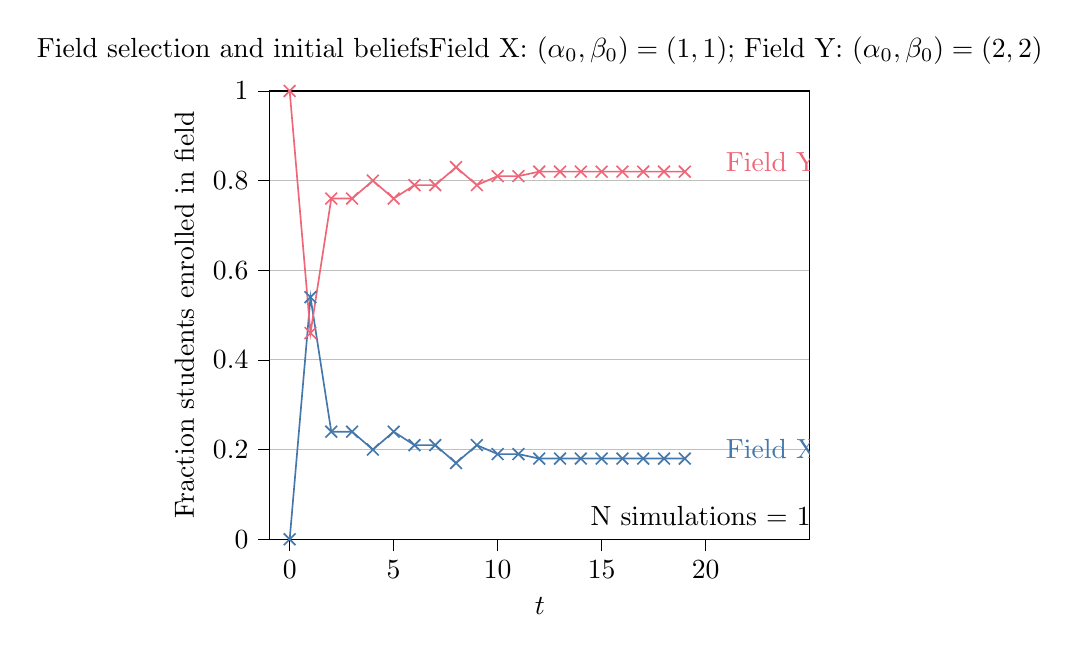
\begin{tikzpicture}

\definecolor{color0}{rgb}{0.266666666666667,0.466666666666667,0.666666666666667}
\definecolor{color1}{rgb}{0.933333333333333,0.4,0.466666666666667}

\begin{axis}[
height=207pt,
tick align=outside,
tick pos=left,
title={Field selection and initial beliefs \\ Field X: \(\displaystyle (\alpha_0, \beta_0)=(1, 1)\); Field Y: \(\displaystyle (\alpha_0, \beta_0)=(2, 2)\)},
width=240pt,
x grid style={white!69.0196078431373!black},
xlabel={\(\displaystyle t\)},
xmin=-0.95, xmax=25,
xtick style={color=black},
xtick={0,5,10,15,20},
xticklabels={\(\displaystyle 0\),\(\displaystyle 5\),\(\displaystyle 10\),\(\displaystyle 15\),\(\displaystyle 20\)},
ylabel={Fraction students enrolled in field},
ymajorgrids,
ymin=0, ymax=1,
ytick style={color=black},
ytick={0,0.2,0.4,0.6,0.8,1},
yticklabels={\(\displaystyle 0\),\(\displaystyle 0.2\),\(\displaystyle 0.4\),\(\displaystyle 0.6\),\(\displaystyle 0.8\),\(\displaystyle 1\)}
]
\addplot [semithick, color0, mark=x, mark size=3, mark options={solid}]
table {%
0 0
1 0.54
2 0.24
3 0.24
4 0.2
5 0.24
6 0.21
7 0.21
8 0.17
9 0.21
10 0.19
11 0.19
12 0.18
13 0.18
14 0.18
15 0.18
16 0.18
17 0.18
18 0.18
19 0.18
};
\addplot [semithick, color1, mark=x, mark size=3, mark options={solid}]
table {%
0 1
1 0.46
2 0.76
3 0.76
4 0.8
5 0.76
6 0.79
7 0.79
8 0.83
9 0.79
10 0.81
11 0.81
12 0.82
13 0.82
14 0.82
15 0.82
16 0.82
17 0.82
18 0.82
19 0.82
};
\draw (axis cs:20.5,0.18) node[
  anchor=base west,
  text=color0,
  rotate=0.0
]{Field X};
\draw (axis cs:20.5,0.82) node[
  anchor=base west,
  text=color1,
  rotate=0.0
]{Field Y};
\draw (axis cs:14,0.03) node[
  anchor=base west,
  text=black,
  rotate=0.0
]{N simulations = 100};
\end{axis}

\end{tikzpicture}
